% ****** Start of file apssamp.tex ******
%
%   This file is part of the APS files in the REVTeX 4.2 distribution.
%   Version 4.2a of REVTeX, December 2014
%
%   Copyright (c) 2014 The American Physical Society.
%
%   See the REVTeX 4 README file for restrictions and more information.
%
% TeX'ing this file requires that you have AMS-LaTeX 2.0 installed
% as well as the rest of the prerequisites for REVTeX 4.2
%
% See the REVTeX 4 README file
% It also requires running BibTeX. The commands are as follows:
%
%  1)  latex apssamp.tex
%  2)  bibtex apssamp
%  3)  latex apssamp.tex
%  4)  latex apssamp.tex
%
\documentclass[%
 reprint,
% superscriptaddress,
%groupedaddress,
%unsortedaddress,
%runinaddress,
%frontmatterverbose, 
%preprint,
%preprintnumbers,
%nofootinbib,
%nobibnotes,
%bibnotes,
 amsmath,amssymb,
 aps,
 prl,
%pra,
% prb,
% rmp,
%prstab,
%prstper,
%floatfix,
]{revtex4-2}

\usepackage{graphicx}% Include figure files
\usepackage{dcolumn}% Align table columns on decimal point
\usepackage{bm}% bold math
\usepackage{blindtext}
\usepackage{float}
\usepackage{caption}
\usepackage{cleveref}
\usepackage{subcaption}
\usepackage{xcolor}
%\usepackage{hyperref}% add hypertext capabilities
%\usepackage[mathlines]{lineno}% Enable numbering of text and display math
%\linenumbers\relax % Commence numbering lines

%\usepackage[showframe,%Uncomment any one of the following lines to test 
%%scale=0.7, marginratio={1:1, 2:3}, ignoreall,% default settings
%%text={7in,10in},centering,
%%margin=1.5in,
%%total={6.5in,8.75in}, top=1.2in, left=0.9in, includefoot,
%%height=10in,a5paper,hmargin={3cm,0.8in},
%]{geometry}


\newcommand{\etal}{{\it et al.}~}
\newcommand{\bom}{\boldsymbol{\omega}}

% \newcommand{\sd}[3][\null]{\ensuremath{\dfrac{\d^{#1} #2}{\d #3^{#1}}}}%Standard derivative 
% \newcommand{\pd}[3][\null]{\ensuremath{\dfrac{\partial^{#1} #2}{\partial #3^{#1}}}}%Partial derivative
% \newcommand{\matd}[2][\null]{\ensuremath{\dfrac{\mathrm{D}^{#1} #2}{\mathrm{D} t^{#1}}}} %Material derivative

\def \s{\mathbf{s}}
\def \v{\mathbf{v}}
\def \x{\mathbf{x}}
\def \r{\mathbf{r}}
\def \k{\mathbf{k}}
\def \h{\mathbf{h}}

\def \cm{\mathrm{cm}}
\def \cms{\mathrm{cm/s}}
\def \sec{\mathrm{s}}
\def \K{\mathrm{K}}

\def\red#1{\textcolor{red}{#1}}
\def\blue#1{\textcolor{blue}{#1}}
\def\magenta#1{\textcolor{magenta}{#1}}


%%%%%%%%%%%%%%%%%%%%%%%%%%%%%%%%%
\newcommand*{\NOTE}[1]{\textbf{\color{red}[#1]}}
\newcommand*{\CHANGE}[1]{{\color{brown}#1}}
\newcommand*{\DEL}[1]{{\color{green}#1}}


\begin{document}

\preprint{APS/123-QED}

%\title{Inverse energy transfer in finite-temperature superfluid vortex reconnections}
\title{Inverse energy transfer in three-dimensional quantum vortex flows}

\author{P. Z. Stasiak}
\author{A. Baggaley}
\author{C.F. Barenghi}
\affiliation{School of Mathematics, Statistics and Physics, Newcastle University, Newcastle upon Tyne, NE1 7RU, United Kingdom}

\author{G. Krstulovic}
\affiliation{Universit\'e C\^ote d'Azur, Observatoire de la C\^ote d'Azur, CNRS,Laboratoire Lagrangre, Boulevard de l'Observatoire CS 34229 - F 06304 NICE Cedex 4, France}

\author{L. Galantucci}
\affiliation{Istituto per le Applicazioni del Calcolo ``M. Picone" IAC CNR, Via dei Taurini 19, 00185 Roma, Italy}

\date{\today}% It is always \today, today,
             %  but any date may be explicitly specified

\begin{abstract}
Vortex reconnections play a fundamental role in fluids.
% and they are typically considered as a mechanism to 
They increase the complexity of flow and develop small-scale motions.
In this work, we report that in superfluids, they can also excite large scales.
We numerically illustrate that during a superfluid vortex reconnection energy 
is injected 
into the thermal (normal) component of helium~II at small length scales, but is transferred nonlinearly  to larger length scales, increasing the integral length scale of the normal
fluid.  
We show that this inverse energy transfer is triggered by the helical imbalance generated 
%at reconnection 
in the normal fluid flow by
the mutual friction force coupling the superfluid vortices and the normal component. We finally discuss
%by decomposing the velocity and the mutual friction (which couples superfluid and normal fluid) into helical modes, showing 
%that the imbalance of homochiral modes results from the punctuated energy and helicity injection during the reconnection. Finally, we discuss 
the relevance of our findings to 
the problem of superfluid turbulence.
\end{abstract}

%\keywords{Suggested keywords}%Use showkeys class option if keyword
   %display desired
\maketitle


\begin{figure*}
	\centering
    \begin{subfigure}[b]{0.24\textwidth}
		\centering
		\includegraphics*[width=\textwidth]{snap-1.pdf}
	\end{subfigure}
	\begin{subfigure}[b]{0.24\textwidth}
		\centering
		\includegraphics*[width=\textwidth]{snap-2.pdf}
	\end{subfigure}
    \begin{subfigure}[b]{0.24\textwidth}
		\centering
		\includegraphics*[width=\textwidth]{snap-3.pdf}
	\end{subfigure}
    \begin{subfigure}[b]{0.24\textwidth}
		\centering
		\includegraphics*[width=\textwidth]{snap-4.pdf}

	\end{subfigure} \hfill
    %
	\begin{subfigure}[b]{0.24\textwidth}
		\centering
		\includegraphics*[width=\textwidth]{snaps-hel-1.pdf}
	\end{subfigure}
	\begin{subfigure}[b]{0.24\textwidth}
		\centering
		\includegraphics*[width=\textwidth]{snaps-hel-2.pdf}
	\end{subfigure}
    \begin{subfigure}[b]{0.24\textwidth}
		\centering
		\includegraphics*[width=\textwidth]{snaps-hel-3.pdf}
	\end{subfigure}
    \begin{subfigure}[b]{0.24\textwidth}
		\centering
		\includegraphics*[width=\textwidth]{snaps-hel-4.pdf}
	\end{subfigure} \hfill
	\caption{
Three-dimensional rendering of the time evolution of
an initially orthogonal vortex configuration 
undergoing a vortex reconnection at $T = 1.9$K at dimensionless
times (from left to right)
$(t-t_R)/\tau_R=-7.47\times10^{-2}$, $-3.09\times10^{-3}$, $8.79\times10^{-4}$ and $5.39\times10^{-3}$, where $\tau_R = E^{1/2}_R/ L_R$. The green
tubes represent the superfluid vortex lines (the tubes’ radii have been 
greatly exaggerated for visual purpose). In the top sequence,
the blue volume rendering represents the scaled normal fluid enstrophy 
$\bom^2/\bom^2_{max}$. Note the Kelvin wave on the superfluid
vortex at $(t-t_0)/\tau_R=8.79\times10^{-4}$ . In the bottom sequence, the red/blue volume
rendering at the same times represent scaled positive/negative normal fluid
helicity.	
%Three-dimensional rendering of an orthogonal vortex configuration 
%undergoing a vortex reconnection at $T=1.9K$. The red tubes represent
%the superfluid vortex
%lines (the tubes' radii have been greatly exaggerated for visual purposes), 
%and the blue volume rendering represents the scaled normal fluid enstrophy 
%$\bom^2/\bom^2_{max}$. In the third panel, note the Kelvin waves on the superfluid vortices.
}
    \label{fig:visualisation}
\end{figure*}

%\paragraph*{Introduction.---} 
Turbulence is ubiquitous in the universe.  It occurs in systems
as large as nebulae of interstellar gas, and as small as clouds of
few thousands atoms confined by lasers in the laboratory.
Turbulence shapes patterns and properties of fluids of all
kinds, from ordinary
 viscous fluids (Navier-Stokes turbulence\cite{frisch1995}) 
to electrically conducting fluids (magneto-hydrodynamics turbulence
\cite{canuto-dalsgaard-1998}) to quantum fluid
(quantum turbulence \cite{barenghi-etal-2023,
Barenghi_Skrbek_Sreenivasan_2023}).
All turbulent systems are characterised by 
the existence of a wide range 
of length scales across which inviscid conserved quantities 
are transferred without loss in the spirit of the cascade 
depicted by Richardson \cite{richardson1922weather}. 

In three-dimensional (3D) classical fluids, turbulence 
is characterised by a direct cascade: the
non-linear dissipationless transfer of kinetic energy from the scale of
the large eddies (at which energy is injected) to the smallest length scales
at which energy is dissipated into heat
\cite{richardson1922weather,kolmogorov-1941}. 
The resulting distribution of energy across length scales is
the celebrated Kolmogorov energy spectrum 
\cite{kolmogorov-1941,frisch1995}. 

Confining Navier-Stokes turbulence to two-dimensions (2D) entails 
fundamentally distinct physics: a dual cascade emerges of energy and enstrophy 
(mean squared vorticity) \cite{kraichnan-1967,boffetta-ecke-2012}, 
the two conserved quantities in ideal two-dimensional flows.
% \magenta{(in
%three dimensions the conserved quantities are energy and helicity)}. 
%In particular, while 
While the enstrophy cascade is direct (from large to small
scales), the energy cascade is inverse (from small to large scales)
\cite{boffetta-musacchio-2010}. This inverse cascade 
may favour the generation and persistence of large coherent 
structures \cite{laurie-etal-2014}. 

Remarkably, the same cascade phenomenology is observed in turbulent flows 
of quantum fluids, {\textit{i.e.} fluids at very low temperatures whose physics is
dominated by quantum effects.
Examples of such fluids are superfluid helium 
and atomic Bose-Einstein Condensates (BECs). 
The dynamics of these systems can be successfully depicted in terms of 
a two-fluid model \cite{tisza-1938,landau-1949,skrbek-sreenivasan-2012} 
describing the quantum fluid as the mixture of two components, 
the superfluid component and the thermal (or normal) component, which 
interact by means of a mutual friction force 
\cite{jackson-etal-2009,hall-vinen-1956a,hall-vinen-1956b}. 
The superfluid component flows without viscosity and
vanishing entropy; its vorticity is
confined to effectively one-dimensional vortex filaments
of atomic core thickness (called quantum vortices or vortex lines), 
around which the circulation of the velocity is quantised.
In BECs the thermal component forms a ballistic gas,
whereas in superfluid $^4$He it can be described as
a classical viscous fluid.
Despite these significant differences with respect to ordinary fluids, 
the direct
%forward 
kinetic energy cascade has
indeed been observed in three-dimensional superfluid
turbulence 
\cite{maurer1998,salort2010turbulent,baggaley2012,sherwin-robson2015,Muller_KolmogorovKelvinWave_2020,Muller_IntermittencyVelocityCirculation_2021}.
Evidence of this 
%forward 
direct
cascade has been found also in
three-dimensional turbulent BECs \cite{middleton-spencer2022}. Similarly to 2D classical turbulence, 
an inverse energy cascade characterises turbulence in two-dimensional BECs, 
as shown in theoretical \cite{bradley2012energy,reeves2013,simula2014emergence,Muller_ExploringEquivalenceTwoDimensional_2024} and experimental \cite{johnstone2019evolution,gauthier2019giant} studies.

In turbulent systems, the type and the number of sign-defined ideal invariants determine the direction of cascades. Indeed, the famous 
%and simple 
Fjørtoft argument \cite{fjortoft1953changes} predicts 
the existence of an inverse energy cascade
in 2D classical turbulence. 
%Similarly, for 3D wave-turbulent 3D BECs, the Fjørtoft argument predicts 
It also predicts an inverse particle and a direct energy cascade 
for 3D wave turbulent BECs, as recently addressed theoretically \cite{Zhu_DirectInverseCascades_2023}. In 3D classical fluids, helicity, which is also an inviscid invariant, is not sign-defined and thus only a direct energy cascade is possible. However, recent studies have demonstrated that the direction of the energy 
cascade may be inverted by artificially controlling the chirality of the 
flow, \textit{i.e.} the balance between positive and negative helical 
modes \cite{moffatt1969}.
%, eventually making helicity almost a sign defined quantity. 
Indeed, by restricting the non-linear energy transfer to homochiral 
interactions via a suitable decimation of the Navier-Stokes equation 
\cite{biferaleInverseEnergyCascade2012a,biferale-etal-2013}, by
controlling the weight of homochiral interactions \cite{sahoo-etal-2017},
or by the external injection 
of positive helical modes at all length scales 
\cite{plunianInverseCascadeEnergy2020a}, inverse energy cascades 
have been observed in three-dimensional turbulence of classical fluids. 
In brief, when the flow is synthetically designed to have an 
enhanced chirality, an inverse energy cascade can observed.


In this work, we unveil a similar dynamics occurring in superfluid helium
($^4$He) as a result of vortex reconnections.  
Reconnections occur continuously in turbulence: they take place when
two vortex lines collide and recombine, exchanging heads and tails, 
altering the overall topology of the flow
\cite{koplik-levine-1993,bewley-etal-2008,rorai-etal-2016,serafini-etal-2017,galantucci-baggaley-parker-barenghi-2019,villoisUniversalNonuniversalAspects2017,villois2020irreversible}. 
We show that the mutual friction force arising from the  
vortex reconnection is chiral, injecting in the normal fluid prevalently 
helicity of a given sign. Thus, as a consequence of vortex reconnections,
we observe an increase of the chiral imbalance of the quantum fluid, producing a transfer of kinetic energy from small to large scales, similarly to the phenomenology observed in 3D helical-decimated classical flows. 
 Unlike classical fluids, such a chiral imbalance arises naturally as physical process in the normal fluid.% because of vortex reconnections. 
%This is contrast to classical fluid dynamics,  where the helical characteristics of the flows producing 
% an inverse energy transfer require a careful synthetic construction 
% \cite{biferaleInverseEnergyCascade2012a,biferale-etal-2013,sahoo-etal-2017,plunianInverseCascadeEnergy2020a}.

% WE ADD REFERENCE TO OUR FIRST PAPER LATER IN THE TEXT
%Punctuated energy injection resulting from the violent nature of vortex reconnections \cite{stasiak2024quantum} pave the way for an imbalance of chirality by multi-scale energy injection.
%

%% THIS PART IS TOO DETAILED OF WHAT WE WILL DO AT THIS STAGE, ALTHOUGH PART OF IT MIGHT BE USED IN THE ABSTRACT
%We will show that energy is injected at the small length scales immediately in the post reconnection regimes and moves towards larger length scales, increasing the integral length scale $\mathcal{L}_E$ of the normal fluid component. We provide an explanation of the inverse energy transfer by decomposing the velocity and mutual friction fields (the governing interaction force between the two-fluid components) into helical modes, showing that the imbalance of homochiral modes resulting from the punctuated energy and helicity injection during the reconnection process. Finally, we discuss the relevance of our findings to the broader field of transitions to superfluid turbulence. 

%\paragraph*{Main results.---} 



To model superfluid helium dynamics, we employ the recently developed FOUCAULT model
\cite{galantucciNewSelfconsistentApproach2020b}.  In this approach, superfluid vortex lines are
parametrized as one-dimensional space curves  $\s(\xi,t)$, $\xi$ and $t$ being arclength and time respectively, exploiting the large separation of length scales between the vortex core radius, the Lagrangian discretisation along the vortex lines $\Delta\xi$, and the average radius of curvature $R_c$ of the vortex lines. The vortex lines evolve according to the following equation of motion:
\begin{equation}
    \dot{\s}(\xi,t) = \v_s + \frac{\beta}{1+\beta}\left[\v_{ns}\cdot\s'\right]\s' + \beta\s'\times\v_{ns} + \beta'\s'\times\left[\s'\times\v_{ns}\right],
\end{equation}
where $\dot{\s} = \partial\s/\partial t$, $\s' = \partial\s/\partial\xi$ is the unit tangent vector, $\v_n$ and $\v_s$ are the normal fluid and superfluid velocities at $\s$, $\v_{ns} = \v_n-\v_s$, and $\beta,\, \beta'$ are temperature and Reynolds number dependent mutual friction coefficients \cite{galantucciNewSelfconsistentApproach2020b}. The calculation of the superfluid velocity $\v_s$ is performed via the computation of the Biot-Savart integral de-singularised with standard techniques (see Supplementary Material \cite{suppMat}). The normal fluid is described classically using the incompressible ($\nabla\cdot\v_n=0$) 
Navier-Stokes equation
\begin{equation}
    \frac{\partial\v_n}{\partial t} + (\v_n\cdot\nabla)\v_n = -\frac{1}{\rho}\nabla p  + \nu_n\nabla^2\v_n + \frac{\mathbf{F}_{ns}}{\rho_n} \; \; , 
\end{equation}
%
where $\rho_n$ and $\rho_s$ are the normal fluid and superfluid densities,
$\rho=\rho_n + \rho_s$,  $p$ is the pressure,  $\nu_n$ is the kinematic 
viscosity of the normal fluid, and the mutual friction force per unit
volume, $\mathbf{F}_{ns}$, is the line integral of the mutual friction 
force per unit length, $\mathbf{f}_{ns}$ \cite{suppMat}:
%
\begin{equation}
\mathbf{F}_{ns}(\x) = 
\oint_{\mathcal{C}}\delta(\x-\s)\mathbf{f}_{ns}(\s)d\xi,     
\end{equation}
$\mathcal{C}$ representing the entire vortex configuration. 
The regularisation of mutual friction is performed using a physically self-consistent scheme \cite{galantucciNewSelfconsistentApproach2020b}. %, gualtieri2015exact, gualtieri2017turbulence}. 
We consider a periodical box of size $2\pi$ (so that  wavevectors are integers).

To study the reconnection dynamics, we consider two pairs of initially orthogonal vortices (where the corresponding vortices of each pair have opposite circulation in order to preserve periodicity along the boundaries)
at two distinct temperatures, $T=1.9K$ and $T=2.1K$. The vortex pairs are separated by the distance $D_{\ell}$; each vortex within each pair is initially at distance $d_{\ell}$ to the other vortex, such that $d_{\ell}\ll D_{\ell}$ to ensures that the dynamics in the vicinity of the reconnection is dominated by local interactions, and that the far-field contribution from the other vortex pair is negligible.

The evolution of the vortex reconnection of a single pair is reported in Fig.~\ref{fig:visualisation}. 
The first row shows the reconnecting superfluid vortices (in green) accompanied by normal fluid structures generated by mutual friction, here displayed as enstrophy rendering $\bom(\x)^2=|\nabla\times \v_n|^2$. Such structures are the signature of the violent irreversible energy transfers in vortex reconnections 
\cite{stasiak2024quantum}. The second row shows the rendering of the local helicity $H(\x)=\v_n\cdot\bom$, where we observe a clear local helicity production, with an abrupt change of sign due to the rearrangement of the vortex topology. Remarkably, during reconnection there is a net 
sudden normal fluid helicity production, as shown in Fig.~\ref{fig:total-helicity}. We will come back to this finding later.
\begin{figure}[t]
    \centering
    \includegraphics*[width=0.48\textwidth]{helicity_total}
\caption{Temporal evolution of the normal fluid helicity $\mathcal{H} = \int_{\mathcal{V}}H(\x)dV$ computed over the entire volume $\mathcal{V}$. For superfluid helium, it is proper to make the helicity dimensionless in terms of $\kappa^2$. The quantities $E_R$ and $L_R$ are the energy $E$ and integral length scales $L_0$ of the normal fluid at reconnection time $t_R$.}
\label{fig:total-helicity}
\end{figure}

We now focus on the time evolution of the normal fluid energy spectrum $E(k)$, defined by 
\begin{equation}
    E = \frac{1}{(2\pi)^3}\int_{\mathcal{V}}\frac{1}{2}|\v_n|^2 dV = \int_0^{\infty}E(k)dk
\end{equation}
where $E$ is the total normal fluid energy and $k$ is the magnitude of the three-dimensional wavenumber. The energy at reconnection $E_R$ is given by $E(t_R)$, where $t_R$ is the time at reconnection. The energy spectrum $E(k)$ is displayed in Fig.~\ref{fig:kinetic-energy}.
\begin{figure}[h!]
    \centering
    \begin{subfigure}{0.49\textwidth}
        \centering
        \includegraphics*[width=\textwidth]{energy-spec.pdf}
        \caption{}\label{fig:kinetic-energy}
    \end{subfigure}
    \begin{subfigure}{0.49\textwidth}
        \centering
        \includegraphics*[width=\textwidth]{flux-spec.pdf}
        \caption{}\label{fig:energy-flux}
    \end{subfigure}
    \caption{\emph{(a):} Normal fluid kinetic energy spectrum $E(k)$ before 
reconnection (dashed lines), at reconnection (solid lines) 
and after reconnection (dotted lines) for $T=1.9K$ (red)
and $T=2.1K$ (blue).\emph{(b):} Spectral normal fluid kinetic energy flux, $\Pi (k)$. It is normalised using the integral scale and the normal fluid energy at reconnection.
\emph{Inset:} Post reconnection evolution of the integral length scale, $L_0$.
Times and temperatures are labelled as in Fig.~\ref{fig:kinetic-energy}.}
\end{figure}
%

It clearly emerges that, during the reconnection, energy is predominantly injected into the normal fluid at intermediate and small length scales. 
For $k>5$ in correspondence of the reconnection time $t_R$,
we observe a significant increase of the normal fluid energy spectral density:
$E(k,\, t\approx t_R)/E(k,\, t\ll t_R) \approx 10^2$. 
%
In the post-reconnection regime, we simultaneously observe a small 
decrease of the spectrum at intermediate 
and small scales ($k > 5$) and an increase at large scales, 
suggesting the existence of a mechanism by 
which energy generated at small length scales is transferred to larger scales. 
To shed light on this mechanism, as customary for turbulent flows, we analyse the spectral energy flux 
\begin{equation}
    \Pi(k)=\int_{|{\bf p}|<k}  \hat{\mathbf{v}}_n^*\cdot \left [\widehat{(\v_n\cdot\nabla)\v_n} \right ]d {\bf p} +c.c. \;\; ,
\end{equation}
where $\widehat{\cdot}$ indicates the Fourier transform.

% the dynamics of the normal fluid flow using the 
% spectral energy budget equation: 
% %
% \begin{equation}
%     \frac{\partial E(k)}{\partial t} = T(k) - D(k) + I(k)
% \end{equation}
% where $T(k)$ is the spectral kinetic energy transfer function,
% %(\textit{i.e.} $T(k)dk$ is the energy transfered per unit time by modes with $k < |\mathbf{k}| < k +dk$, determined by non-linear effects), 
% $D(k)=2\nu_n k^2 E_k$ is the dissipation spectrum and
% %=\mathrm{Re}(\hat{\mathbf{F}}_{ns}(\k)\cdot\hat{\v}^*(\k))$ 
% $I(k)$ is the injection spectrum arising from the mutual friction 
% force $\mathbf{F}_{ns}$.  
We observe that $\Pi(k) < 0$ for all $k$ during and after reconnection;
we also observe that, near the time of reconnection,
the peak value of $|\Pi(k)|$ is in the range $15 < k < 25$.
%
The negative sign of $\Pi(k)$ is evidence of a flux of kinetic  energy from small to large scales, exciting larger and larger scales. % In other words, at non-zero temperatures,
% vortex reconnections trigger an inverse transfer of energy, 
% which implies the creation of large scale structures, visible
% in Fig.~\ref{fig:visualisation}} \NOTE{GK: the figure shows small scale structures...}
This behaviour is quantified by the evolution of the integral length scale $L_0$, defined as
\begin{equation}
    L_0 = \frac{\pi}{2 E}\int_0^{\infty}\frac{E(k)}{k}dk, %\Big/ \int_0^{\infty}\!\!E(k)dk.
\end{equation}
The inset of Fig.~\ref{fig:energy-flux} shows that
$L_0$ indeed  increases steadily in the post-reconnection regime. Note that times have been normalised by the largest eddy-turnover-time at the reconnection event, evidencing  it fast evolution.

To explain the inverse energy transfer shown in Fig.~\ref{fig:kinetic-energy},
we look whether the reconnection triggers a chirality imbalance. 
We decompose the incompressible Fourier modes of the normal fluid velocity 
into helical modes \cite{waleffe-1992}:
\begin{equation}
\hat{\mathbf{v}}_n (\k) = \hat{\mathbf{v}}_n^+(\k) +\hat{\mathbf{v}}_n^-(\k)=
 v_n^+(\mathbf{k}) \mathbf{h}^+(\mathbf{k})+v_n^-(\mathbf{k}) \mathbf{h}^-(\mathbf{k}),
\end{equation}
%
where $\mathbf{h}^\pm (\mathbf{k})$ are the two eigenvectors of the curl 
operator, \textit{i.e.} $i\k~\times~\h^{\pm}(\k)~=~\pm k \h^{\pm}(\k)$. 
Similarly, we decompose the transverse modes of the mutual friction force:
$\hat{\mathbf{F}}_{ns}^{\perp}(\k) = f^+(\k) \mathbf{h}^+ + f^-(\k) \mathbf{h}^-$
(the  Fourier modes of $\mathbf{F}_{ns}$ parallel to the wavemumber 
$\k$ do not play any role in the time evolution of $\mathbf{v}_n$ 
due to the incompressible constraint). Finally, the helical decomposition naturally allow us decompose the total helicity as $\mathcal{H}=\mathcal{H}^+-\mathcal{H}^-$ \cite{plunianInverseCascadeEnergy2020a}.
% %
% The spectral energy densities corresponding to the helical modes are
% $E^{\pm}(\k) = (1/2) |v_n^\pm(\k)|^2$, the total spectral density 
% being $E(\k) = E^{+}(\k) + E^{-}(\k)$. Similarly the spectral helicity 
% density is 
% \begin{equation}
% \begin{split}
% H(\k) & = (1/2) \hat{\mathbf{v}}_n (\k)\!\!\! ~\cdot~\!\!\! \hat{\bm{\omega}}_n^* (\k) = \\
% & = k E^+(\k) - k E^-(\k)  = H^+(\k) - H^-(\k),
% \end{split}
% \end{equation}
% where $\bm{\omega}_n$ is the normal fluid vorticity, the star indicates 
% complex conjugate and $H^\pm$ is the helicity contribution of each 
% separate helical mode. \NOTE{GK: the standard definition of the energy and helicity spectra contains the sum over the angles, so the previous definition are wrong (except if you redifined them for some reason).}
%The rate of change $I^\pm(\k)$ of the energies $E^{\pm}(\k)$ arising from the mutual friction is proportional to the corresponding helical coefficients $f^\pm$, \textit{i.e.} $I^\pm(\k) = \mathrm{Re} [f^\pm (v_n^\pm)^*] /\rho_n$, and the related signed helicity injection is $I_H^\pm(\k) = k \mathrm{Re} [f^\pm (v_n^\pm)^*] /\rho_n$. 

A chiral imbalance occurs if the mutual friction force is helical, 
\textit{i.e.} if the ratio $|f^+|^2/|f^-|^2 \neq 1$, with $|f^\pm|^2$ the total squared norm of the mutual friction components. 
In Fig.~\ref{fig:mutual-friction-decomp}, we show the temporal evolution of $|f^+|^2/|f^-|^2$, for both temperatures. 
%
\begin{figure}[h!]
    \centering
    \includegraphics*[width=0.48\textwidth]{fmfDecompFig.pdf}
    \caption{Temporal evolution of projected mutual friction force components $f^\pm$/ Inset: temporal evolution of total helical components.}.
    \label{fig:mutual-friction-decomp}
\end{figure}
%
It is apparent
that during and after the reconnection, the mutual friction force is strongly chiral,
injecting more negative helicity than positive helicity. 
As a result, the ratio $\mathcal{H}^+/\mathcal{H}^-$ 
(reported in the inset of Fig.~\ref{fig:mutual-friction-decomp}) 
decreases significantly at reconnection and remains smaller than unity even at later times, 
indicating that the flow is persistently chiral. We conclude that the reconnection triggers indeed a chiral imbalance.
From Fig.~\ref{fig:mutual-friction-decomp} we determine the non-dimensional timescale $\tau = (t^*-t_R)E_R^{1/2}/L_R$
during which the mutual friction force is chiral as a result of reconnections: $\tau \approx 0.01$ and $\tau \approx 0.005$
for $T=1.9$K and $T=2.1$K, respectively, corresponding dimensionally to $\tau \approx 0.1$s for both temperatures. 
In superfluid turbulence, the timescale between two consecutive reconnections can be smaller than $\tau$ provided that the
vortex line density $\mathcal{L}$ (length of vortices per unit volume) is larger than $10^8 \text{m}^{-2}$ \cite{stasiak2024quantum,barenghi2004},
a condition which is easily met in superfluid helium experiments \cite{roche2007,Babuin2014}.


%Furthermore, as observed in
%Ref.~\cite{plunianInverseCascadeEnergy2020a}, to observe a negative energy flux the forcing needs to cover the entire spectrum of $k$, which  from the inset of Fig.~\ref{fig:kinetic-energy}, it is evident that this indeed the case.


  

%we follow recent work in classical fluids outlined in Refs.~\cite{biferaleInverseEnergyCascade2012a,plunianInverseCascadeEnergy2020a}, where it is even possible to sustain an inverse energy cascade under a helical forcing applied at all length scales. Typically, velocity coefficients $\hat{\v}(\k)$ can be decomposed into their helical modes, where $\hat{\v}(\k)=v^+(\k)\h^+(\k) + v^-(\k)\h^-(\k)$ and satisfies $\k\cdot\hat{\v}(\k)=0$, where $\v^{\pm}$ are complex scalars and $\h^{\pm}(\k)$ are the two eigenvectors of the curl operator, such that $i\k\times\h^{\pm}(\k)=\pm k \h^{\pm}(\k)$. To explain the inverse energy transfer in terms of helical modes, we show that in fact the driving force, which in our case is a punctuated burst due to superfluid vortex reconnections, is of a helical nature. The mutual friction modes $\hat{\mathbf{F}}_{ns}(\k)$ are not incompressible, and so we take the projection of the modes orthogonal to the wavenumber $\k$. The projected modes $\hat{\mathbf{f}}(\k)$ are then decomposed into helical modes $\hat{\mathbf{f}}(\k)=f^+\h^{+}(\k) + f^-\h^{-}(\k)$. The ratio of the two helical modes $|f^+|^2/|f^-|^2$ are shown in Fig.~\ref{fig:mutual-friction-decomp}. At reconnection time $t_0$, the ratio is much larger, indicating that indeed this force is chiral and that a clear inbalance that favours the injection of positive helical modes, changing the chirality of the flow (as seen in Fig.~\ref{fig:mutual-friction-decomp}). In the same way, helicity modes $\hat{\mathcal{H}}(\k)$ can be decomposed,
%\begin{equation}
%    \hat{\mathcal{H}}(\k) = k(E^+(\k) - E^-(\k)) = \mathcal{H}^+ + \mathcal{H}^-
%\end{equation}
%where $E^{\pm}=\frac{1}{2}|\v^{\pm}(\k)|^2$ are the helical energy modes. The evolution of the ratio $\mathcal{H}^+/\mathcal{H}^-$ is shown in the inset of Fig.~\ref{fig:mutual-friction-decomp}. The sharp increase at reconnection time $t_0$ is evidence of a large influx of positive helical modes as a result of the vortex reconnection, which is in agreement with the conditions to facilitate an inverse energy transfer by a helical injection. Finally, as observed in Ref.~\cite{plunianInverseCascadeEnergy2020a}, it is necessary for the forcing to cover the entire spectrum of $k$, which from the inset of Fig.~\ref{fig:kinetic-energy}, it is evident that this indeed the case.           

%\paragraph*{Closing remarks.---}
In conclusion, the reconnection of quantum vortices in the two-fluid regime
($T\gtrsim 1.5$K) not only injects punctuated
energy in the normal fluid \cite{stasiak2024quantum}, but also triggers in the normal fluid
a transfer of kinetic energy towards the large scales. 
%This inverse 
%energy transfer arises from the fact that the mutual friction force (injecting energy and 
%helicity in the normal fluid) is helical, as Kelvin waves develop on the vortices as a result of the reconnection itself.
%The helical character of the mutual friction produces a chiral imbalance in the normal fluid, driving this inverse transfer, as previously observed in turbulent Navier-Stokes flows
This inverse energy transfer arises from the helical character of the
friction generated by the Kelvin waves released by the reconnecting
cusp, which produces a chiral imbalance in the normal fluid, as 
previously observed in turbulent Navier-Stokes flows
\cite{biferaleInverseEnergyCascade2012a,plunianInverseCascadeEnergy2020a}.

Our findings have profound implications for the nature of turbulence in 
finite temperature superfluids. In circumstances where the vortex density 
$\mathcal{L}$ is large and where the isotropy of the vortex tangle 
is broken by external forcing, the chirality of the flow generated by the 
frequent reconnections may be strong enough to induce an inverse energy 
cascade \cite{notes_recon}.
%The asymmetry of the reconnecting vortex configurations is a key element; 
%when perfectly symmetrical vortex configurations (with corresponding 
%opposite vortex line orientations) reconnect, the injected helicity 
%globally cancels out, as verified in our study if we take also into 
%account the reconnection.
The microscopic mechanism that we have described is probably what
triggers the inverse energy cascade which is observed numerically in  
large-scale simulations of counterflow turbulence at large heat fluxes \cite{polanco2020}, which
indeed inherently not isotropic.
%, hence triggering non-fully reconnections. 
Our work hence motivates further detailed studies of
the role played by helicity in superfluid dynamics 
\cite{dileoni2016,galantucci2021},
moving the emphasis from few vortex systems \cite{scheeler2014} 
to fully coupled superfluid turbulence.
 




\begin{acknowledgments}
    G.K. was supported by the Agence Nationale de la Recherche through the project the project QuantumVIW ANR-23-CE30-0024-02.
    This work has been also supported by the French government, through the UCAJEDI Investments in the Future project managed by the National Research Agency (ANR) with the reference number ANR-15-IDEX-01. P.Z.S. acknowledges the financial support of the UniCA ``visiting doctoral student program'' on complex systems. Computations were carried out at the Mésocentre SIGAMM hosted at the Observatoire de la Côte d’Azur.

  \end{acknowledgments}


\bibliography{references}% Produces the bibliography via BibTeX

\appendix
\section*{Supplementary Materials}

Using Schwarz mesoscopic model \cite{schwarz1988}, vortex lines can be described as space curves $\s(\xi,t)$ of infinitesimal thickness, with a single quantum of circulation $\kappa=h/m_4=9.97\times10^{-8}\text{m}^2/\text{s}$, where $h$ is Planck's constant, $m_4=6.65\times10^{-27}\text{kg}$ is the mass of one helium atom, $\xi$ is the natural parameterisation, arclength, and $t$ is time. These conditions are a good approximation, since the vortex core radius of superfluid \textsuperscript{4}He($a_0=10^{-10}\text{m}$) is much smaller than any of the length scales of interest in turbulent flows. The equation of motion is
\begin{equation}
	\dot{\s}(\xi,t) = \v_s + \frac{\beta}{1+\beta}\left[\v_{ns}\cdot \s'\right]\s' + \beta\s'\times\v_{ns}+\beta'\s'\times\left[\s'\times \v_{ns}\right],
\end{equation}
where $\dot{\s}=\partial\s/\partial t$, $\s'=\partial\s/\partial \xi$ is the unit tangent vector, $\v_{ns}=\v_n - \v_s$, $\v_n$ and $\v_s$ are the normal fluid and superfluid velocities at $\s$ and $\beta$,$\beta'$ are temperature and Reynolds number dependent mutual fricition coefficients \cite{galantucciNewSelfconsistentApproach2020b}. The superfluid velocity $\v_s$ at a point $\x$ is determined by the Biot-Savart law
\begin{equation}
	\v_s(\x,t) = \frac{\kappa}{4\pi}\oint_{\mathcal{T}}\frac{\s'(\xi,t)\times\left[\x-\s(\xi,t)\right]}{|\x-\s(\xi,t)|}d\xi,
\end{equation}
where $\mathcal{T}$ represents the entire vortex configuration.
There is currently a lack of a well-defined theory of vortex reconnections in superfluid helium, like for the Gross-Pitaevskii equation \cite{villois2020irreversible,villoisUniversalNonuniversalAspects2017,promentMatchingTheoryCharacterize2020a}. An \emph{ad hoc} vortex reconnection algorithm is employed to resolve the collisions of vortex lines \cite{baggaleySensitivityVortexFilament2012a}.

\begin{figure}
	\centering
	\begin{subfigure}[b]{0.49\textwidth}
		\centering
		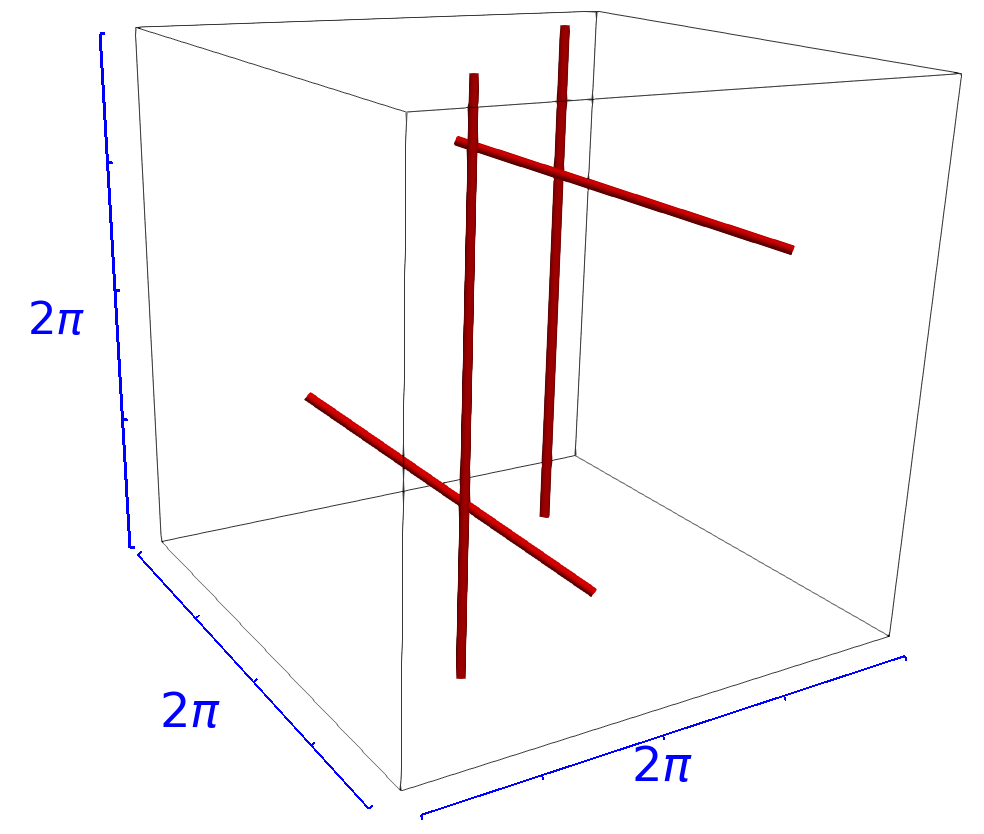
\includegraphics[width=0.8\textwidth]{schematic.png}
	\end{subfigure}
	\begin{subfigure}[b]{0.49\textwidth}
		\centering
		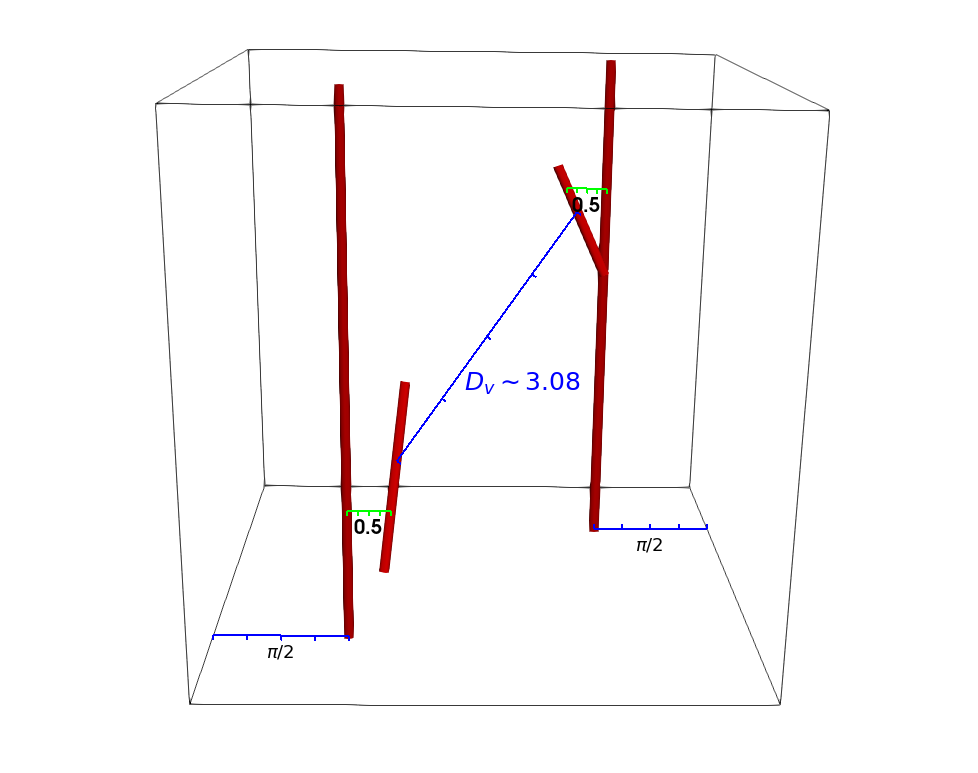
\includegraphics[width=0.9\textwidth]{schematic-2.png}
	\end{subfigure}
	\caption{Schematic diagram of the initial vortex configuration.}
	\label{fig:schematic}
\end{figure}

A \emph{two-way model} is crucial to understand the accurately interept the back-reaction effect of the normal fluid on the vortex line and vice-versa \cite{stasiak2024quantum}. We self-consistently evolve the normal fluid $\v_n$ with a modified Navier-Stokes equation
\begin{equation}
	\frac{\partial \v_n}{\partial t} + (\v_n\cdot\nabla)\v_n = -\nabla\frac{p}{\rho} + \nu_n\nabla^2\v_n + \frac{\mathbf{F}_{ns}}{\rho_n},
\end{equation}
\begin{equation}
	\mathbf{F}_{ns} = \oint_{\mathcal{T}}\mathbf{f}_{ns}\delta(\x-\x)d\xi, \quad \nabla\cdot\v_n=0,
\end{equation}
where $\rho=\rho_n + \rho_s$ is the total density, $\rho_n$ and $\rho_s$ are the normal fluid and superfluid densities, $p$ is the pressure, $\nu_n$ is the kinematic viscosity of the normal fluid and $\mathbf{f}_{ns}$ is the local friction per unit length \cite{galantucciCoupledNormalFluid2015a}
\begin{equation}
	\mathbf{f}_{ns} = -\mathcal{D}\s'\times\left[\s'\times(\dot{\s}-\v_n)\right]-\rho_n\kappa\s'\times(\v_n-\dot{\s}), 
	\label{eq:mutual-friction}
\end{equation}
where $\mathcal{D}$ is a coefficient dependent on the vortex Reynolds number and intrinsic properties of the normal fluid. The regularisation of the mutual fricition force onto the normal fluid grid is physically motivated by the strongly localised injection of vorticity during the momentum exchange of point-like particles and viscous flow in classical fluid dynamics \cite{gualtieri2015exact,gualtieri2017turbulence}. In short, the localised vorticity induced by the relative motion between the vortex lines and the normal fluid is diffused to discretisation of the grid spacing $\Delta x$ in a time interval $\epsilon_R$. In this way, the delta-forced fricition as defined in Eq.~\ref{eq:mutual-friction} is regularised by a Gaussian function, the fundamental solution of the diffusion equation. Further details of the method for classical fluids are contained in \cite{gualtieri2015exact,gualtieri2017turbulence} and for FOUCAULT in \cite{galantucciNewSelfconsistentApproach2020b}.  



In this Letter, we report all results using dimensionless units, where the characteristic length scale is $\tilde{\lambda} = D/D_0$, where $D^3=(1\times10^{-3}\mathrm{m})^3$ is the dimensional cube size, $D_0^3=(2\pi)^3$ is the non-dimensional cubic computational domain. The time scale is given by $\tilde{\tau}=\tilde{\lambda}^2\nu_n^0\nu_n$, where the non-dimensional viscosity $\nu_n^0$ resolves the small scales of the normal fluid. In these simulations, these quanties are $\tilde{\lambda}=1.59\times10^{-4}$m, $\nu_n^0=0.32$ and $\tilde{\tau}=0.366$s at $T=1.9K$ and $\tilde{\tau}=0.485$s at $T=2.1K$. We consider an initial configuration of two pairs of orthongal vortices, initialised as shown in the schematic of Fig.~\ref{fig:schematic}. The seperation between vortices in each pair $d$ is set to be $d_v=0.5$ in dimensionless units, and the shortest distance between pairs is $D_v=\sqrt{(\pi-d_v/2)^2+\pi^2}\approx 3.08$, so that $d_v\ll D_v$. The Lagrangian discretisation of vortex lines is $\Delta \xi = 0.025$ (a total of 1340 discretisation points across the 4 vortex lines), using a timestep of $\Delta t_{VF} = 5.56\times10^{-6}$. For the normal fluid, a total of $N=256^3$ mesh point were used, with a timestep of $\Delta t_{NS} = 45\Delta t_{VF}$. 

\end{document}
%
% ****** End of file apssamp.tex ******
